

%%%%%%%%%%%%%%%%%%%%%%%%%%%%%%%%%%%%%%%%%%%%%%
\section{Muon Tagger}
\label{sec:beam:muontagger}

%%%%%%%%%%%%%%%%%%%%%%%%%%
\subsection{Overview}

The ProtoDUNE-SP muon tagger, called the Cosmic Ray Tagger (CRT), enables tagging and reconstruction of muons crossing the TPC volume. It is intended to provide a sample of tracked comic-ray muons (and beam halo muons), with known $t0$'s, to map out the effects of space charge, which are expected to be large. It will also aid in measuring the electron lifetime in the TPC.

The ProtoDUNE-SP CRT is an assembly of highly segmented scintillator-strip modules and readout electronics that were originally built for the Double Chooz large-area muon-tagging system, called the Outer Veto.  
 
The modules have been fully tested %following construction at the University of Chicago, 
and are currently stored relatively close to CERN in Strasbourg. The PMTs and front-end electronics %, originally produced at Columbia University, 
require shipping from %are stored at 
Virginia Tech.

Whereas the Double Chooz Outer Veto modules are installed horizontally above the detector, ProtoDUNE-SP arrays the modules in panels that are oriented vertically and installed on the upstream and downstream sides of the detector, as shown in Figure~\ref{fig:crt-panel-placement}. 

\begin{cdrfigure}[Placement of upstream and downstream Cosmic Ray Tagger (CRT) panels]{crt-panel-placement}{Placement of upstream (left) and downstream (right) CRT panels with respect to the detector. Each panel consists of eight modules  (light green). This shows a possible assembly in which the upstream side has two panels and the downstream side has one. Full coverage of the detector faces would require eight four-module units. The panels can be moved laterally along the support structure shown.}
  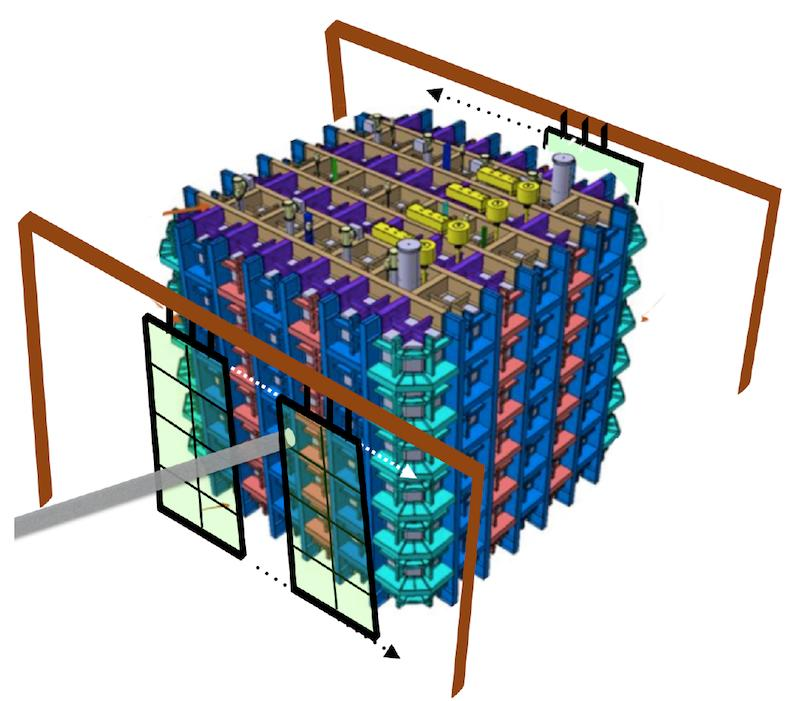
\includegraphics[width=0.6\textwidth]{crt-panel-placement}
\end{cdrfigure}


%%%%%%%%%%%%%%%%%%%%%%%%%%
\subsection{CRT module design and readout}

The CRT module design is illustrated in Figure~\ref{fig:one-crt-module}. Each module contains 64 5-cm wide $\times$ 1-cm thick $\times$ 320-cm long scintillator strips in two 32-strip layers; the strips in both layers are parallel to each other, and offset by half a strip width. This provides an effective pitch of 2.5\,cm.

\begin{cdrfigure}[Drawing of Cosmic Ray Tagger (CRT) module]{one-crt-module}{Drawing of one 64-strip CRT module (one 32-strip layer shown).  Each module contains two layers of 32 5-cm $\times$ 1-cm $\times$ 320-cm strips with wavelength-shifting fibers.  The 64 fibers for each module are coupled to a Hamamatsu M64.}
  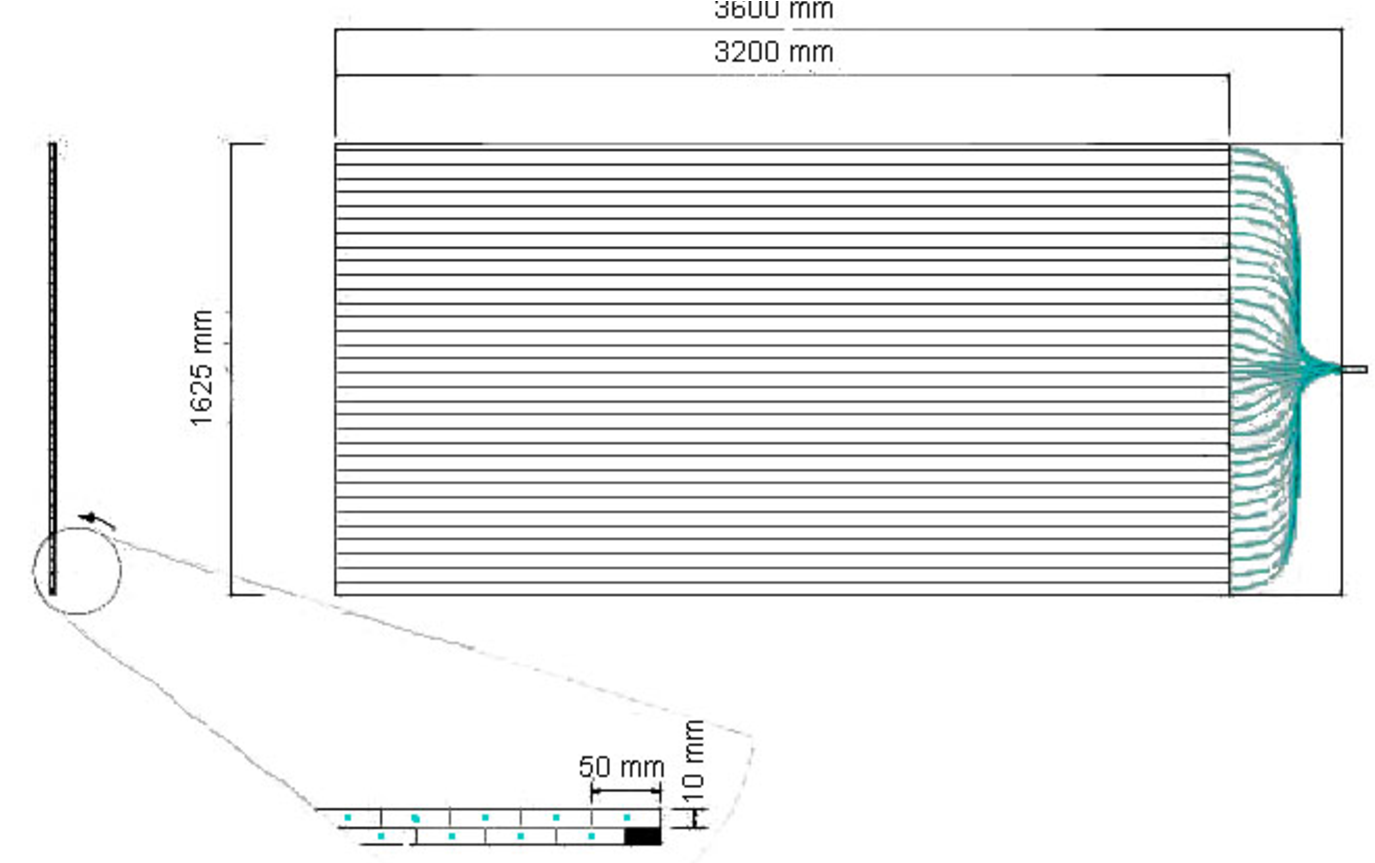
\includegraphics[width=0.6\textwidth]{one-crt-module}
\end{cdrfigure}


Each scintillator strip has a 1.5-mm diameter wavelength-shifting fiber inserted into a hole created during the extrusion process.   Given the space required for the fiber routing at the end, %, and the 2.5-cm offset, t
the resulting modules are 3.6-m long, 162.5\,cm wide and about 2\,cm thick. The modules are covered with aluminum as shown in Figure~\ref{fig:crt-module-photo}). 


\begin{cdrfigure}[Photo of CRT module]{crt-module-photo}{Photo of CRT module. The inset shows the front-end board attached to the PMT and module. The two large chips are the MAROC2 and an Altera FPGA.}
  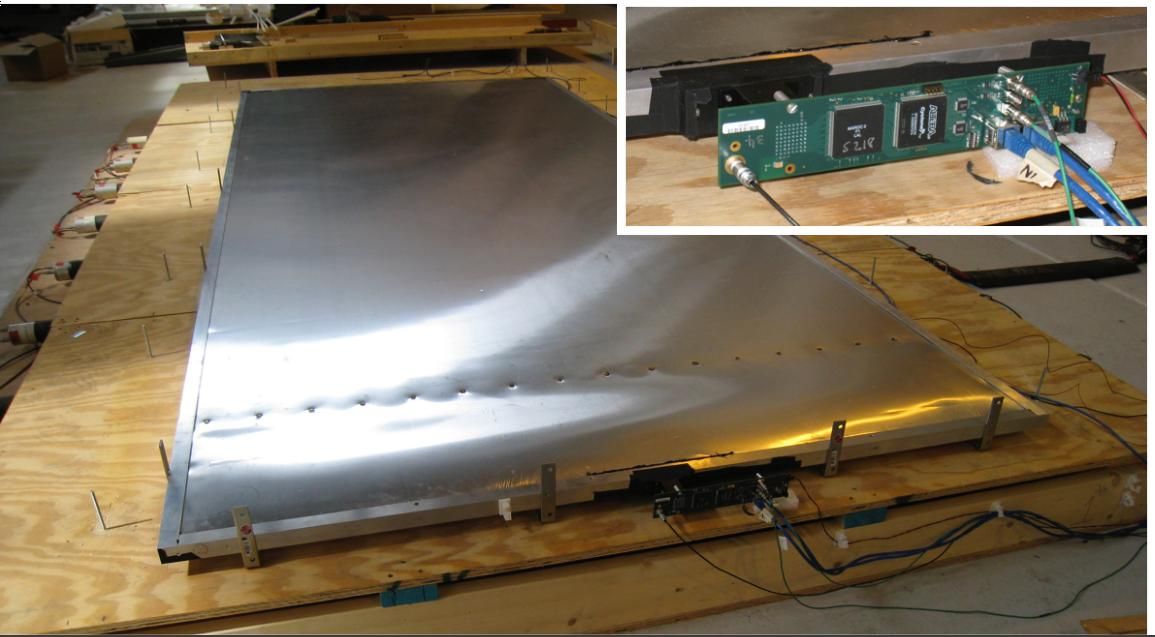
\includegraphics[width=0.7\textwidth]{crt-module-photo.jpg}
\end{cdrfigure}


The 64 wavelength-shifting fibers on one end (right-hand side of  Figure~\ref{fig:one-crt-module})
are coupled to a Hamamatsu M64 multi-anode photomultiplier tube (PMT); the other fiber ends are mirrored for reflection. 
Each M64 is connected to a custom front-end board with a MAROC2 ASIC and an FPGA as shown in the inset of Figure~\ref{fig:crt-module-photo}.
The MAROC2 allows adjustment of the electronic gain of each of the 64 channels; this is needed to correct for the factor-of-two pixel-to-pixel gain variation in the M64.  Signals that exceed a common threshold are sent to a multiplexed 12-bit ADC, providing pulse height information for hit strips. The readout of each module is self-triggered. Each module requires a 62.5-MHz clock and a sync pulse. The sync pulse is a NIM signal with
a frequency between 0.5 and 0.05\,Hz. The sync signal is used to reset the internal counter of each module. 
Each module produces a single NIM trigger output indicating the presence of a muon-like signal (i.e., overlapping hits in the two module layers).


%%%%%%%%%%%%%%%%%%%%%%%%%%
\subsection{Layout of CRT modules}

The ProtoDUNE-SP CRT is based on units of four modules, layered and oriented orthogonally as shown in Figure~\ref{fig:four-module-layout}). These four-module units result in a 3.2-m $\times$ 3.2-m area.  Figure~\ref{fig:crt-layout} is a photograph of an actual unit.

\begin{cdrfigure}[Orthogonal layout of a four-module CRT unit]{four-module-layout}{Illustration of orthogonal layout of a four-module CRT unit, providing 2D readout. Two modules are in back (landscape orientation in diagram), with the inactive portion for the fibers, PMTs, and readout electronics at right; two modules are in front (portrait orientation), with the inactive portion at the top. A support structure sits between the front and back modules (grey and brown grid); additional support is provided on both outside surfaces by structures that clamp the modules to the inside support. The outer support for the front modules is shown in green.}
  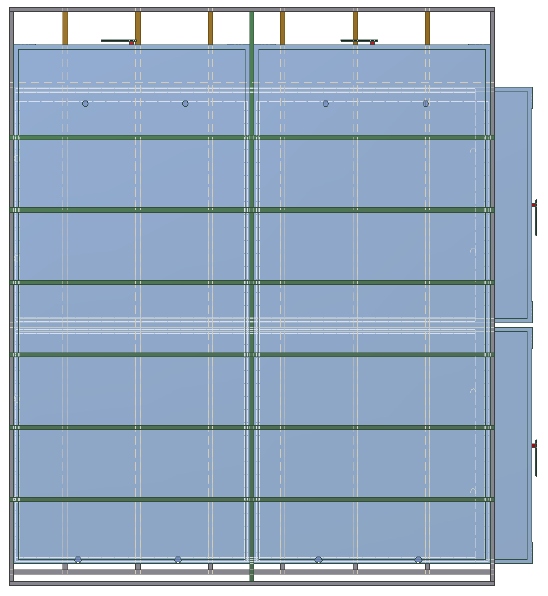
\includegraphics[width=0.5\textwidth]{four-module-layout}
 \end{cdrfigure}


\begin{cdrfigure}[Photo of four-module CRT unit from Double Chooz]{crt-layout}{Photo of fully assembled four-module layout at Double Chooz. The top modules are oriented lower right to upper left in the photo; the inactive portions of the bottom modules can be seen in the lower left and center.}
  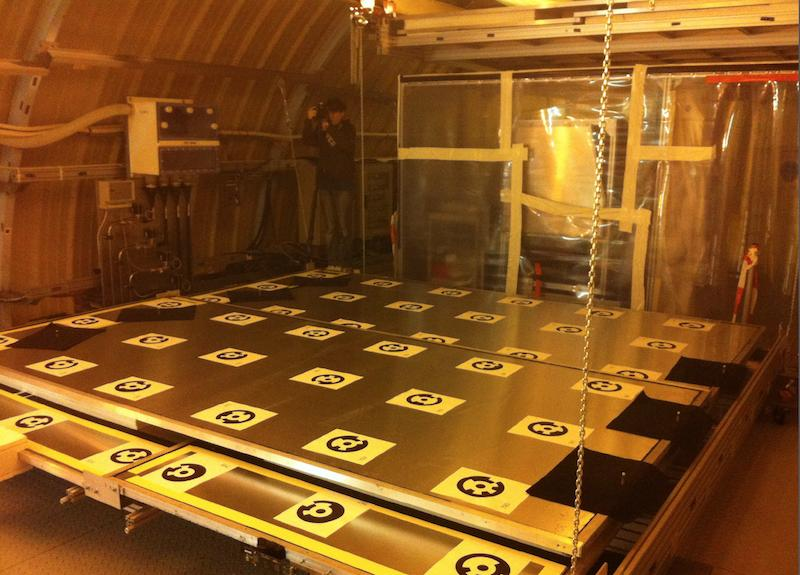
\includegraphics[width=0.7\textwidth]{double-chooz-layout}
\end{cdrfigure}

Tests are currently underway to evaluate two schemes for holding the modules. Following these small-scale tests, a full prototype structure with a real module will be constructed and tested in Chicago.

Possible locations for modules parallel to the upstream and downstream faces of the cryostat are under investigation. %Modules on these faces enable tagging and reconstruction of muons crossing the TPC volume. 
%Full coverage of these faces, which would require eight four-module units, would allow field distortions to be mapped over the full TPC volume. 
The CRT installation must preserve access to the outside of the cryostat, either by leaving sufficient fixed space between the detector and the panels or by sliding panels out of the way. 
The panels must also avoid existing infrastructure. An appealing option for the upstream face is to make use of some of the existing APA rails. It is anticipated that a rails-and-hanger system identical to the APA design for both the upstream and downstream CRT modules will be used, as illustrated in Figure~\ref{fig:crt-panel-placement}. In the possible arrangement shown in the figure, which employs 24 modules (six four-module units), data is taken with the downstream modules first in one position then the other, to cover the full TPC volume.


%%%%%%%%%%%%%%%%%%%%%%%%%%
%\subsection{Module position survey} section removed; more detail than needed. ok with Ed B.


%%%%%%%%%%%%%%%%%%%%%%%%%%
\subsection{DAQ and readout}

The CRT uses its own readout. This readout produces a series of ADC values and time stamps for hit strips, and makes use of a ProtoDUNE-SP global clock and sync pulse to enable merging with TPC information -- pseudo-online -- using time stamps. Note that the entire CRT system is isolated from the detector ground; it uses the building ground.

%%%%%%%%%%%%%%%%%%%%%%%%%%
\subsection{Testing of modules during installation}

All modules, PMTs, and front-end readout boards have been fully tested. Prior to installation, QA/QC procedures identical to those used for the Double Chooz installation will be used. Each module is first equipped with a reference PMT and front-end board. Using the same well-characterized PMT + readout board for all modules allows efficient checking for light leaks and other module defects. Once the light-tightness and proper function of the module is verified, the final PMT and PMT board are installed. The function of the PMT/PMT-board combination and the light-tightness of the PMT installation is checked before the module is put into position.
